% !TEX root = ../sparsity_thesis.tex
\chapter{Research Methodology}
\label{ch:methodology}

This chapter describes the methodology by which the research questions
formulated in Chapter~\ref{ch:introduction} were operationalised into a
reproducible empirical study. The chapter follows the canonical
CRISP-DM-aligned sequence of \emph{problem scoping}, \emph{data gathering},
\emph{data preparation}, \emph{modelling}, \emph{evaluation}, and
\emph{deployment}, adapted to the specific concerns of measuring explanation
fidelity rather than predictive accuracy alone.

\section{Problem Scoping}
\label{sec:problem-scoping}

\subsection{Research Objectives}
\label{subsec:meth-objectives}

In direct continuation of Chapter~\ref{ch:introduction}, this research pursues
four objectives, which together translate the abstract research questions
(RQ1--RQ3) into actionable engineering targets:

\begin{enumerate}
    \item \textbf{Quantify XAI degradation under data sparsity.} Establish,
    through controlled cross-sectional experimentation, the empirical
    relationship between tenant-level training-data volume and the fidelity
    and stability of post-hoc SHAP and LIME explanations.
    \item \textbf{Identify the cold-start XAI threshold.} Determine the
    data-volume boundary at which local post-hoc explanations cease to be
    operationally reliable, characterising the non-linear \emph{Reliability
    Cliff} hypothesised in Chapter~\ref{ch:literature-review}.
    \item \textbf{Design the Maturity-Aware AI Routing architecture.} Specify
    a tenant-aware tier-logic gate that conditions the choice of explanation
    strategy on each tenant's data maturity.
    \item \textbf{Implement and evaluate the tier-logic gate.} Realise the
    proposed pattern as a concrete software component inside the studied
    Django / PostgreSQL ERP, and verify that it routes correctly and preserves
    backward compatibility.
\end{enumerate}

\subsection{Research Scope}
\label{subsec:meth-scope}

The methodological scope of this study was constrained as follows in order to
preserve interpretability and reproducibility:

\begin{itemize}
    \item \textbf{Platform.} A single multi-tenant ERP system based on
    Django~4.2 and PostgreSQL, configured under the database-per-tenant
    isolation model.
    \item \textbf{Prediction tasks.} Three ERP-native supervised tabular
    classification problems: Late Delivery Risk prediction, Lead Scoring, and
    Employee Attrition.
    \item \textbf{XAI techniques.} Two post-hoc, model-agnostic explainers
    were evaluated: SHAP (specifically the \emph{TreeExplainer} and
    \emph{LinearExplainer} variants) and LIME (in its tabular form).
    Intrinsically interpretable models and gradient-based explainers for deep
    networks were not within scope.
    \item \textbf{Evaluation mode.} Offline, cross-sectional simulation
    against curated open-source datasets. No live SaaS tenant traffic was
    used, and no longitudinal observation of data accumulation over real
    calendar time was performed.
    \item \textbf{Architectural pattern.} Only the Maturity-Aware AI Routing
    pattern was implemented and evaluated; alternative remedies for sparsity
    (transfer learning, federated learning, meta-learning) were noted but
    deferred to future work.
\end{itemize}

\subsection{Research Contribution}
\label{subsec:meth-contribution}

Two distinct but interdependent contributions emerge from this methodology:

\begin{enumerate}
    \item \textbf{An empirical contribution.} The study quantifies, for the
    first time in a B2B multi-tenant ERP setting, the degradation of post-hoc
    explanation fidelity as a continuous function of tenant data volume,
    using a coherent panel of metrics (Spearman rank correlation, SHAP
    absolute variance, SHAP entropy, LIME top-$k$ Jaccard similarity). The
    resulting curves localise the \emph{Reliability Cliff} and produce a
    defensible numerical threshold for the cold-start regime.
    \item \textbf{An architectural contribution.} The study delivers the
    \textbf{Maturity-Aware AI Routing} pattern as a concrete, implementable
    software-engineering artefact, instantiated inside a real Django ERP
    codebase. The contribution is not merely conceptual: it includes the
    routing rule, its empirically-derived threshold, the global-heuristic
    fallback artefact, and the integration discipline by which the gate is
    added without disturbing the existing ML production code path.
\end{enumerate}

\section{Data Gathering}
\label{sec:data-gathering}

\subsection{Open-Source ERP Datasets}
\label{subsec:datasets}

In the absence of an ethically- and legally-shareable real multi-tenant SaaS
dataset, two well-established open-source corpora were adopted as proxies for
ERP operational data. Both datasets were selected for their structural
similarity to the kinds of tabular, time-stamped, business-process records
that an ERP routinely accumulates.

\paragraph{Olist Brazilian E-Commerce Public Dataset.}
This corpus, released by the Brazilian marketplace platform Olist and hosted
on Kaggle, comprises approximately $100{,}000$ orders placed between 2016 and
2018, distributed across nine relational tables covering customers, sellers,
orders, order items, payments, reviews, and products. After joining the
order, payment, and item tables on the canonical \texttt{order\_id} key, the
resulting unified table contained $N = 96{,}460$ rows. This corpus was used
as the empirical substrate for the \textbf{Late Delivery Risk} prediction
task, operationalised as the binary event ``actual delivery date later than
the estimated delivery date'' (formally,
$\mathbf{1}[\textit{order\_delivered\_customer\_date} >
\textit{order\_estimated\_delivery\_date}]$). The Olist corpus exposes
delivery-time observables but not invoice payment-time observables, so the
literal target is delivery lateness rather than payment lateness; for the
purposes of this study the construct of interest is the wider class of
\emph{ERP-style operational-risk prediction} (sparse, tabular, time-stamped
business-process records with a small positive-class prevalence), of which
late delivery is one instance and late payment is another. The proposed
architectural pattern (Section~\ref{subsec:routing-arch}) is task-agnostic and
generalises directly to the late-payment prediction service
(\texttt{LatePaymentPredictor}) of the studied ERP, which shares the same
tabular, sparsity-conditioned structure.

\paragraph{Synthetic CRM Leads Corpus.}
\label{para:crm-leads-synth}
No public CRM lead-scoring dataset of sufficient size and structural realism
was identified during corpus selection, and the studied ERP's own production
CRM tables could not be released for academic reuse. To enable the
cross-task replication while preserving the methodological invariants of
the Late Delivery Risk experiment (tabular structure, stratified sparsity
gradient, deterministic train/test partitions), a \emph{synthetic CRM
Leads corpus} was generated and stored at
\texttt{datasets/crm\_leads\_dataset.csv}. The corpus contains $N = 5{,}000$
lead records (one row per lead) with $20$ raw columns; after dropping
personally-identifying and post-event fields and one-hot encoding the
categorical attributes \texttt{source}, \texttt{service\_interest},
\texttt{country}, and \texttt{job\_title}, the model-facing feature matrix
comprises $34$ covariates. The binary target is
$\textsf{won} = \mathbf{1}[\textit{status} = \text{\textsf{won}}]$, with a
class prevalence of $21.3\%$ positives.

The four numeric predictors are \texttt{estimated\_value} (deal size),
\texttt{probability} (sales-team-assigned win likelihood at the time of
scoring), \texttt{activity\_count} (count of touchpoints recorded against
the lead), and \texttt{days\_in\_pipeline} (age of the lead since
\texttt{created\_at}). The four categorical predictors are
\texttt{source}, \texttt{service\_interest}, \texttt{country}, and
\texttt{job\_title}.

Three leakage controls are imposed by construction. First, the column
\texttt{conversion\_date} is populated \emph{only} for converted leads and
is therefore a post-event variable that perfectly determines the target;
it is dropped before training. Second, the raw \texttt{status} column is
the target itself and is excluded from features. Third, all
identifier and PII columns (\texttt{lead\_number},
\texttt{first\_name}, \texttt{last\_name}, \texttt{email},
\texttt{phone}, \texttt{mobile}, \texttt{company\_name}, \texttt{city},
\texttt{created\_at}, \texttt{last\_contact\_date}) carry no
predictive content under the chosen feature representation and are
dropped. The resulting feature matrix therefore represents the current
snapshot of a lead at the moment a scoring call would be issued, mirroring
how CRM systems expose lead state to a downstream model in production.

The rationale for using a synthetic corpus is twofold: (i)~it permits full
release of the dataset alongside the simulator script
(\texttt{thesis/scripts/lead\_scoring\_simulator.py}), ensuring exact
reproducibility of the cross-task replication, and (ii)~it allows the same
stratified slicing procedure to be applied with controlled class prevalence
and controlled feature semantics, isolating the sparsity treatment from
confounding distributional drift. The principal limitation is one of
external validity: because the records are drawn from a parametric
generator rather than a real CRM workflow, the absolute level of
predictive performance and the specific feature importances reported in
Chapter~\ref{ch:results} should be read as illustrative of \emph{the
shape of the sparsity-induced degradation curve}, not as point estimates
transferable to any particular commercial CRM deployment. The structural
findings of interest---the monotone collapse of rank agreement, the
order-of-magnitude expansion of attribution variance, and the cold-start
flip of predictive performance---are nevertheless replicated on this
corpus and are interpreted as evidence of the architectural pattern
rather than as production-grade performance estimates.

\paragraph{IBM HR Analytics Employee Attrition Dataset.}
This corpus, released by IBM Watson Analytics, contains $1{,}470$ employee
records labelled with a binary \texttt{Attrition} outcome and 34 covariates
spanning demographic, compensation, tenure, and performance-rating fields. It
was adopted as the empirical substrate for the \textbf{Employee Attrition}
prediction task, which directly corresponds to the HR-attrition use case
inside the ERP's HR module.

The suitability of these datasets as ERP proxies rests on three structural
correspondences: (i)~both are tabular, transactionally-keyed records of
business events; (ii)~both expose covariates whose semantics (timestamps,
monetary amounts, tenure, categorical statuses) match those of typical ERP
fields; and (iii)~the volume of each corpus is large enough to support the
construction of a five-tier sparsity gradient while leaving a held-out
evaluation partition intact.

\section{Data Preparation}
\label{sec:data-prep}

\subsection{Feature Engineering}
\label{subsec:feature-eng}

Each raw record was passed through a deterministic feature-engineering
pipeline that produced 13 engineered covariates per row, grouped into four
families:

\begin{itemize}
    \item \textbf{Temporal-derivative features.} From the raw
    \texttt{order\_purchase\_timestamp},
    \texttt{order\_approved\_at}, and
    \texttt{order\_estimated\_delivery\_date} columns, the variables
    \texttt{approval\_delay\_hours} (purchase-to-approval interval),
    \texttt{estimated\_delivery\_days} (the courier ETA quoted to the
    customer at order time),
    \texttt{purchase\_hour}, and \texttt{purchase\_dow} (day-of-week of
    purchase) were computed.
    \item \textbf{Monetary features.} From the order-items and payments
    tables, the variables \texttt{payment\_value}, \texttt{freight\_value},
    and \texttt{price\_total} (aggregate line-item total per order) were
    derived.
    \item \textbf{Cardinality features.} The variables \texttt{num\_items}
    (line-item count) and \texttt{payment\_installments} (number of
    instalments selected at checkout) were extracted, capturing order-level
    structural complexity.
    \item \textbf{Categorical encodings.} The \texttt{payment\_type} field
    was one-hot encoded into four indicator columns
    (\texttt{credit\_card}, \texttt{boleto}, \texttt{voucher},
    \texttt{debit\_card}).
\end{itemize}

\paragraph{Leakage-avoidance constraint.}
\label{para:leakage-avoidance}
All engineered covariates listed above are restricted, by construction, to
information that would be available at the moment a late-payment prediction
is required---namely, at order approval / invoice issuance. Timestamps from
the delivery pipeline---\texttt{order\_delivered\_carrier\_date} and
\texttt{order\_delivered\_customer\_date}---are reserved \emph{solely} for
the construction of the binary target and are explicitly excluded from the
feature matrix. In particular, an earlier version of this study included
the covariate \texttt{carrier\_delay\_hours}, defined as the interval
between \texttt{order\_approved\_at} and
\texttt{order\_delivered\_carrier\_date}; it was subsequently removed
because, although it precedes the customer-delivery event, it is itself a
delivery-pipeline observable and is therefore not realised at prediction
time in a deployed ERP late-payment workflow. Its inclusion would have
constituted a textbook instance of target leakage and would have inflated
the predictive metrics reported in Chapter~\ref{ch:results} without
reflecting a capability the model would possess in production. The
restriction reduces the engineered feature count from $14$ to $13$ and
rules out the trivial metric inflation that would otherwise arise from
explaining a delivery-time outcome with a delivery-time covariate.

Missing values were imputed using the column-wise median for numeric
features and the modal value for categorical features, and the resulting
matrix was standardised by z-scoring of numeric columns. The binary target
\texttt{is\_late} was constructed as
$\mathbf{1}[\textit{order\_delivered\_customer\_date} >
\textit{order\_estimated\_delivery\_date}]$. The overall positive-class
prevalence after joining was $8.1\%$, establishing a moderately imbalanced
classification problem consistent with typical ERP late-delivery (and, by structural analogy, late-payment) base rates.

\subsection{Multi-Tenant Simulation Strategy}
\label{subsec:multi-tenant-sim}

Because no commercially-shareable multi-tenant ERP dataset exists at the
scale required to expose a sparsity gradient, this study adopted a
\emph{stratified data-volume slicing} strategy to simulate the long-tail
distribution of tenant maturities observed empirically in production SaaS
platforms. The procedure was as follows:

\begin{enumerate}
    \item The unified, feature-engineered Olist late-delivery table
    ($N = 96{,}460$, positive prevalence $8.1\%$) was first partitioned into
    a global hold-out evaluation set ($20\%$, $n = 19{,}292$) using a
    stratified random split with seed $\textsf{SEED} = 42$, preserving the
    late-delivery class prevalence.
    \item From the remaining $77{,}168$ training rows, five disjoint
    \emph{simulated tenant partitions} were drawn by stratified random
    sampling without replacement, each preserving the global positive-class
    prevalence (Table~\ref{tab:tenant-tiers}).
    \item Each tenant partition was subsequently subjected to its own
    internal $80/20$ stratified train/validation split, again with
    $\textsf{SEED} = 42$, yielding tenant-local training and validation folds.
    \item All five tenants were evaluated against the \emph{shared} global
    hold-out evaluation set, so that cross-tenant comparisons of predictive
    performance and explanation fidelity referred to an identical test
    distribution and were therefore directly comparable.
\end{enumerate}

\begin{table}[h]
\centering
\caption{Simulated tenant tiers used in the sparsity experiment.}
\label{tab:tenant-tiers}
\renewcommand{\arraystretch}{1.2}
\begin{tabular}{@{}clrl@{}}
\toprule
\textbf{Tier} & \textbf{Tenant label} & \textbf{Sample size $n$} &
\textbf{Interpretation} \\
\midrule
A & Data-Rich    & 50{,}000 & Mature enterprise tenant \\
B & Medium       &  5{,}000 & Established SME tenant \\
C & Sparse       &  1{,}000 & Onboarded SME tenant \\
D & Very Sparse  &      200 & Newly-active SME tenant \\
E & Cold-Start   &       50 & Just-onboarded SME tenant \\
\bottomrule
\end{tabular}
\end{table}

This stratified slicing strategy is methodologically conservative: by
preserving the class prevalence at every tier, it ensures that any observed
degradation in predictive or explanatory quality at smaller $n$ is
attributable to \emph{data volume}, not to changes in label distribution.
The same procedure was applied, with appropriate sample sizes, to the IBM HR
Attrition corpus.

\begin{figure}[h]
    \centering
    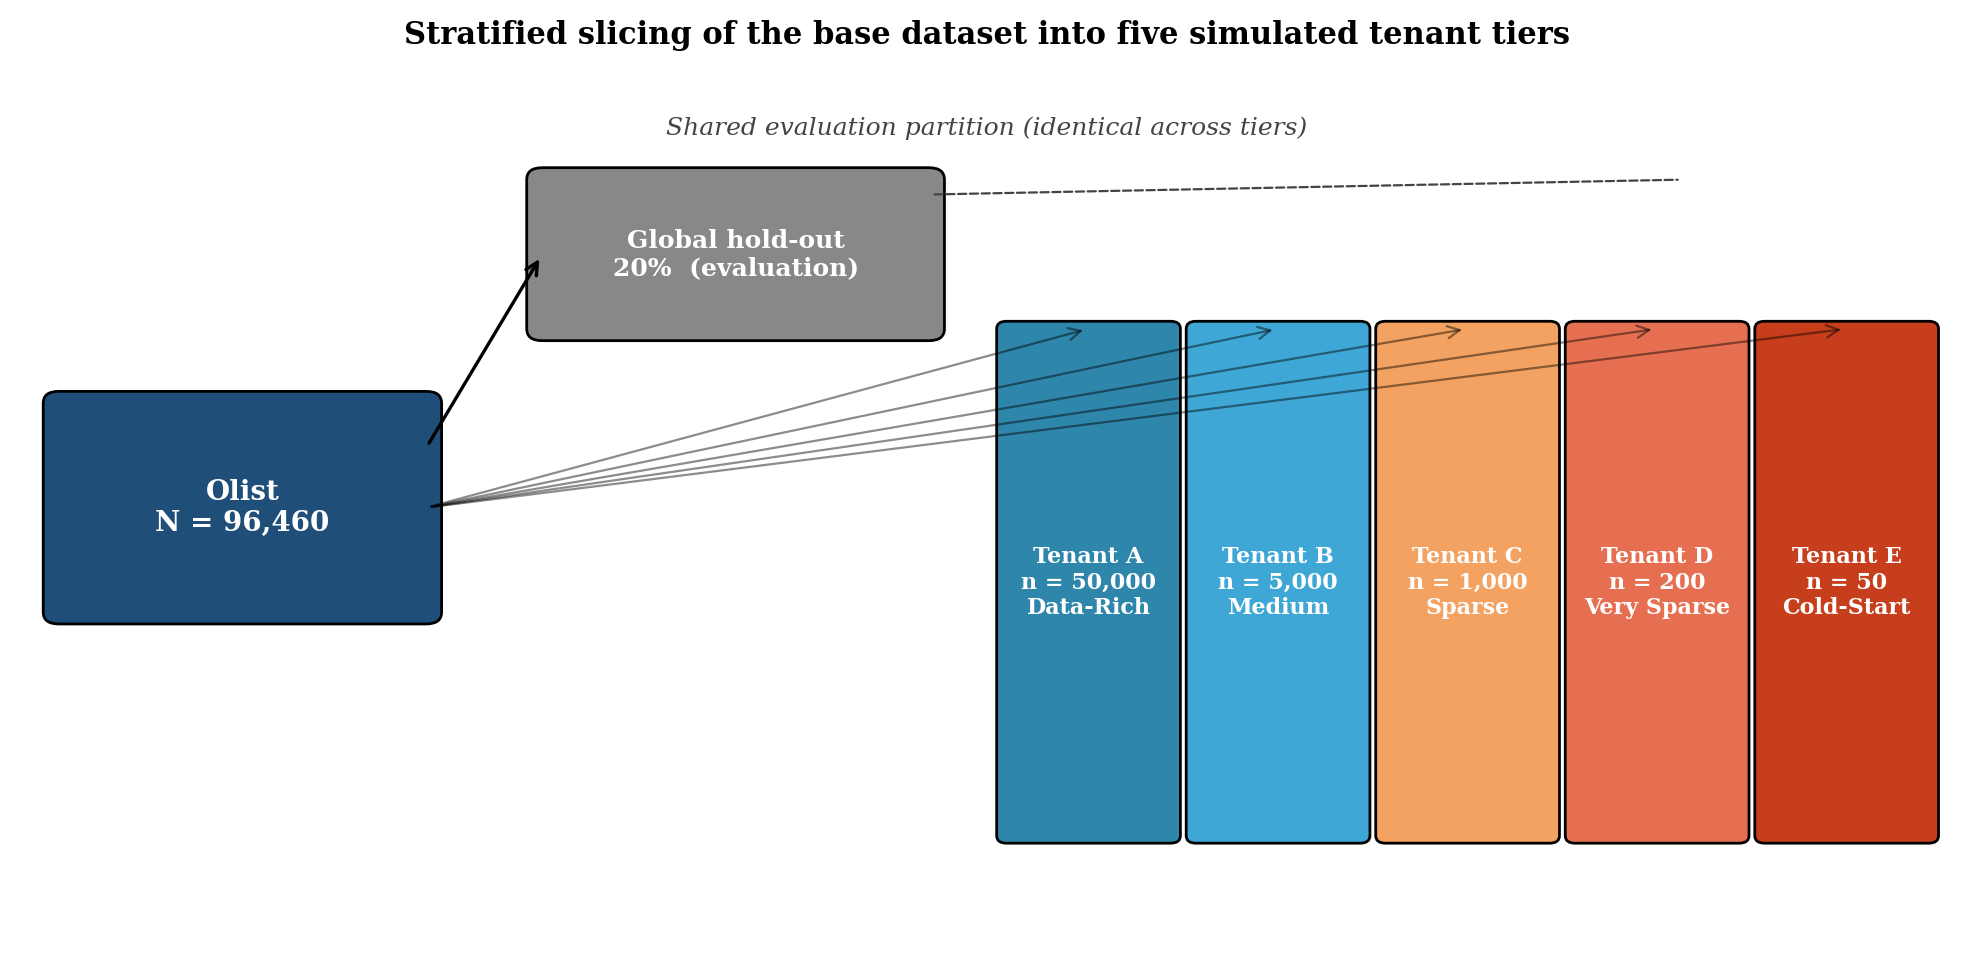
\includegraphics[width=0.95\textwidth]{sparsity_fig_3_1_simulation_strategy.png}
    \caption{Stratified slicing of the base Olist dataset ($N = 96{,}460$)
    into a shared $20\%$ global hold-out evaluation partition and five
    disjoint simulated tenant tiers ($n = 50{,}000$; $5{,}000$; $1{,}000$;
    $200$; $50$), with class prevalence preserved at each tier.}
    \label{fig:sim-strategy}
\end{figure}

\section{Modelling}
\label{sec:modelling}

\subsection{Machine Learning Algorithms}
\label{subsec:algorithms}

Three supervised classifiers were selected, each appropriate to one
prediction task and each representative of a different model family widely
used in operational ERP analytics:

\begin{itemize}
    \item \textbf{Late Delivery Risk --- Gradient Boosting Machine (GBM).}
    Implemented via scikit-learn's \texttt{GradientBoostingClassifier} with
    $n_{\text{estimators}} = 100$, $\textit{max\_depth} = 3$,
    $\textit{learning\_rate} = 0.1$, and the default deviance loss. GBMs were
    selected because tree-ensemble methods are the de facto industry
    standard for tabular financial classification, and because their
    structure is directly compatible with SHAP's polynomial-time
    \emph{TreeExplainer}.
    \item \textbf{Lead Scoring --- Gradient Boosting Machine (GBM).}
    Implemented via scikit-learn's \texttt{GradientBoostingClassifier} with
    $n_{\text{estimators}} = 200$, $\textit{max\_depth} = 3$,
    $\textit{learning\_rate} = 0.05$, and the default deviance loss. The
    same algorithmic family as the Late Delivery Risk task was retained
    deliberately, so that any cross-task differences in the sparsity-induced
    degradation trajectory can be attributed to substrate properties
    (dimensionality, feature dominance, class prevalence) rather than to
    algorithmic confounders. An earlier design used Logistic Regression as a
    representative linear baseline; it was superseded by the GBM variant
    once the replication scope was extended, in order to keep the algorithmic
    surface invariant across tasks and thereby strengthen the
    architectural-pattern claim.
    \item \textbf{Employee Attrition --- Random Forest.} Implemented via
    scikit-learn's \texttt{RandomForestClassifier} with $n_{\text{estimators}}
    = 200$, $\textit{max\_depth} = \text{None}$,
    \texttt{class\_weight = "balanced"}, and \texttt{random\_state = 42}.
    Random forests were chosen for their robustness on small-to-medium
    tabular HR datasets, where the IBM corpus is itself only $1{,}470$ rows.
\end{itemize}

For each prediction task, an identical algorithm was retrained from scratch
on each of the five tenant partitions, producing five independent fitted
models per task. All randomness was controlled via $\textsf{SEED} = 42$ to
guarantee bit-level reproducibility.

\subsection{Explainable AI (XAI) Integration}
\label{subsec:xai-integration}

After fitting, each per-tenant model was subjected to a uniform post-hoc XAI
pipeline:

\begin{itemize}
    \item \textbf{SHAP attribution.} For the tree-based models
    (GBM, Random Forest), SHAP values were computed via the polynomial-time
    \texttt{shap.TreeExplainer}, yielding both per-instance attribution
    vectors and the global mean-absolute-SHAP feature-importance ranking.
    For the Logistic Regression model, \texttt{shap.LinearExplainer} was
    used with the matching background distribution.
    \item \textbf{LIME surrogate explanation.} For every model, local
    explanations were generated using
    \texttt{lime.lime\_tabular.LimeTabularExplainer} configured with
    \texttt{mode="classification"}, $5{,}000$ perturbation samples per
    explanation, and a Gaussian kernel width of $\sqrt{M}$ where $M$ is the
    number of features. The top-$5$ features per instance were retained for
    downstream stability analysis.
    \item \textbf{Sampling for evaluation.} Because LIME is stochastic,
    every LIME-based metric was averaged over $50$ independent runs per
    instance, and SHAP values were always computed on the full shared global
    hold-out set so that cross-tenant comparisons referred to identical
    inputs.
\end{itemize}

This pipeline yields, for each (task, tenant) combination, a paired bundle
consisting of the trained model, the global SHAP feature-importance ranking,
the per-instance SHAP attributions on the hold-out set, and the LIME top-$5$
selections together with their stability statistics.

\subsection{Maturity-Aware AI Routing Architecture}
\label{subsec:routing-arch}

The architectural contribution of the methodology is the
\textbf{Maturity-Aware AI Routing} gate, which conditions the choice of
explanation strategy on the data maturity of the requesting tenant. The
gate was designed around three engineering principles: it must be
\emph{empirically grounded} (its threshold must be derived from the same
experiments that motivate its existence); it must be \emph{architecturally
minimal} (it must not require any change to the existing ML services); and
it must be \emph{fail-safe} (an unavailable global heuristic must not block
predictions).

The routing rule was formalised as follows. Let $n_t$ denote the number of
historically-recorded operational records for tenant $t$ (in the Late
Delivery Risk case, the count of invoices with status in $\{\textit{paid},
\textit{overdue}, \textit{partial}\}$), and let $\tau$ denote the
empirically-derived cold-start threshold. The architectural gate is then:
\begin{equation}
\textsf{explain}(t, x) \;=\;
\begin{cases}
    \textsf{GlobalHeuristic}() & \text{if } n_t \le \tau, \\
    \textsf{LocalShapLime}(t, x) & \text{otherwise.}
\end{cases}
\label{eq:routing}
\end{equation}

The boundary is deliberately \emph{inclusive} on the cold-start side: a
tenant with exactly $n_t = \tau$ records is routed to the global heuristic
rather than to a local explanation. This reflects the empirical finding
(Section~\ref{subsec:threshold}) that Tenant~C ($n = 1{,}000$) already lies
below the $\rho = 0.70$ reliability bound and already exhibits an inflated
SHAP variance, and it removes a latent off-by-one ambiguity in the
route-decision logic. The equivalent code-side formulation
$n_t < \textsf{MIN\_LOCAL\_EXPLANATION\_RECORDS}$ with
$\textsf{MIN\_LOCAL\_EXPLANATION\_RECORDS} = \tau + 1 = 1{,}001$ is
logically interchangeable and may be preferred where a strictly-less-than
guard is idiomatic.

The threshold $\tau$ was not chosen arbitrarily; as detailed in
Section~\ref{subsec:threshold} below, it was identified as $\tau = 1{,}000$
from the empirical fidelity curves derived in the modelling phase. The
threshold was encapsulated in the implementation as a class-level constant
\texttt{COLD\_START\_INVOICE\_THRESHOLD = 1000} (interpreted under the
inclusive boundary above) to allow operational re-tuning without code
change. The two branches of the gate correspond, in
the implementation, to:

\begin{itemize}
    \item \texttt{\_load\_global\_heuristic()} --- a memoised loader that
    reads the pre-computed cross-tenant SHAP feature-importance artefact
    (\texttt{cold\_start\_heuristic.json}, see
    Section~\ref{subsec:heuristic-artifact}) from disk and returns it as a
    structured explanation payload;
    \item \texttt{predict()} --- the existing per-tenant ML inference and
    SHAP/LIME explanation routine, left fully unchanged.
\end{itemize}

The gate itself is exposed as a new public method,
\texttt{predict\_or\_heuristic(invoice)}, which inspects
\texttt{\_invoice\_count()} and dispatches accordingly. The return payload
of both branches conforms to a single response schema (mode, threshold,
count, explanation), so that downstream consumers can be agnostic to which
branch was taken while still being able to surface the routing decision to
the end user.

\begin{figure}[h]
    \centering
    \begin{tikzpicture}[
        node distance=7mm and 10mm,
        every node/.style={font=\footnotesize},
        io/.style={draw,rounded corners=2pt,align=center,inner sep=4pt,
                   minimum width=3.6cm,minimum height=9mm,fill=blue!5},
        proc/.style={draw,align=center,inner sep=4pt,
                     minimum width=4.0cm,minimum height=9mm,fill=gray!8},
        decision/.style={draw,diamond,aspect=2,align=center,inner sep=1pt,
                         minimum width=4.2cm,fill=orange!15},
        outcome/.style={draw,rounded corners=2pt,align=center,inner sep=4pt,
                        minimum width=4.2cm,minimum height=10mm,fill=green!10},
        arr/.style={-{Latex[length=2mm]},thick},
    ]
        \node[io] (req) {Inference request:\\\texttt{predict\_or\_heuristic(invoice)}};
        \node[proc,below=of req] (count) {\texttt{\_invoice\_count()} $\rightarrow n_t$};
        \node[decision,below=of count] (gate) {$n_t \le \textsf{COLD\_START\_INVOICE\_THRESHOLD}$?\\\scriptsize (threshold $= 1{,}000$; inclusive)};
        \node[outcome,below left=10mm and 2mm of gate] (heur)
            {\textbf{Global heuristic}\\\texttt{\_load\_global\_heuristic()}\\\scriptsize reads \texttt{cold\_start\_heuristic.json}};
        \node[outcome,below right=10mm and 2mm of gate] (local)
            {\textbf{Local SHAP/LIME}\\per-tenant \texttt{predict()}\\\scriptsize TreeExplainer + LimeTabular};
        \node[io,below=22mm of gate] (resp) {Response payload\\\scriptsize\{mode, threshold, count, explanation\}};
        \draw[arr] (req) -- (count);
        \draw[arr] (count) -- (gate);
        \draw[arr] (gate.west) -| node[above,pos=0.25,font=\scriptsize] {yes (cold-start)} (heur.north);
        \draw[arr] (gate.east) -| node[above,pos=0.25,font=\scriptsize] {no (data-mature)} (local.north);
        \draw[arr] (heur.south) |- (resp.west);
        \draw[arr] (local.south) |- (resp.east);
    \end{tikzpicture}
    \caption{Maturity-Aware AI Routing architectural gate. The
    \texttt{LatePaymentPredictor.predict\_or\_heuristic()} method inspects the
    tenant's invoice count $n_t$ against the inclusive boundary
    $n_t \le \texttt{COLD\_START\_INVOICE\_THRESHOLD} = 1{,}000$
    (equivalently, $n_t < \textsf{MIN\_LOCAL\_EXPLANATION\_RECORDS} = 1{,}001$).
    Cold-start tenants are dispatched to the global heuristic served from
    \texttt{cold\_start\_heuristic.json}; data-mature tenants are dispatched
    to the per-tenant SHAP/LIME pipeline. Both branches emit a single
    schema-conformant response payload.}
    \label{fig:routing-arch}
\end{figure}

\section{Evaluation}
\label{sec:meth-evaluation}

\subsection{Predictive Performance Metrics}
\label{subsec:pred-metrics}

To establish a baseline against which the explanation-fidelity findings
could be interpreted, the standard panel of predictive metrics was computed
for each (task, tenant) combination on the shared global hold-out set:

\begin{itemize}
    \item \textbf{AUC-ROC} --- the area under the receiver-operating-
    characteristic curve, which is robust to class imbalance and serves as
    the primary headline metric of \emph{predictive} model quality.
    \item \textbf{F1-Score} --- the harmonic mean of precision and recall on
    the positive class, computed at the default $0.5$ probability
    threshold; this metric captures whether the model produces actionable,
    threshold-crossed predictions at all.
    \item \textbf{Brier score} --- recorded as an auxiliary calibration
    diagnostic.
\end{itemize}

These metrics are necessary but not sufficient: a high AUC indicates that
the model has learned a usable signal, but says nothing about whether the
SHAP or LIME explanation of that signal is faithful. The novel contribution
of the evaluation methodology lies in the explanation-fidelity metrics
introduced next.

\subsection{Explanation Fidelity Metrics}
\label{subsec:fid-metrics}

Three complementary metrics were used to convert the abstract notion of
\emph{explanation reliability} into reproducible numerical scores.
Throughout, Tenant~A (the $n = 50{,}000$ data-rich model) is designated as
the \emph{reference baseline}, on the operational premise that of the five
simulated tenants it is the only one whose underlying model can plausibly
be regarded as having recovered the true generative structure.

\paragraph{Spearman Rank Correlation ($\rho$) --- Baseline Rank Agreement.}
Let $r^{A}_i$ denote the rank of feature $i$ in the global mean-absolute-
SHAP importance ranking produced by Tenant~A's model, and let $r^{t}_i$
denote the corresponding rank under tenant $t \in \{B, C, D, E\}$.
Defining $d_i = r^{A}_i - r^{t}_i$, the Spearman rank correlation between
tenant $t$ and the baseline is
\begin{equation}
\rho_t \;=\; 1 \;-\; \frac{6 \sum_{i=1}^{n} d_i^{\,2}}{n\,(n^2 - 1)},
\label{eq:spearman-meth}
\end{equation}
where $n$ is the number of features. By construction, $\rho_A = 1$. A value
$\rho_t \ge 0.70$ is treated, following the explanation-stability
literature, as the operational lower bound of acceptable ranking agreement;
$\rho_t$ values below this threshold are taken as quantitative evidence
that the tenant's local explanation rankings are no longer recovering the
same feature-importance signal as the data-rich baseline.

\paragraph{Construct-validity caveat.}\label{para:rho-caveat}
The metric $\rho_t$ measures \emph{baseline rank agreement} (equivalently,
\emph{reference-aligned explanation stability}) between tenant $t$ and the
data-rich Tenant~A; it is \emph{not} a measure of true explanation fidelity
in the sense of agreement with the data-generating process. Tenant~A is a
reference model, not a ground-truth model: under the leakage-corrected
Late Delivery Risk experiment Tenant~A itself only attains
$\text{AUC} = 0.6556$ and $F_1 = 0.0263$, which is well below the
threshold at which one would attribute oracle status to its attribution
rankings. The interpretation throughout this thesis is therefore
operational: $\rho_t$ quantifies the extent to which a sparsely-trained
tenant's SHAP rankings deviate from those of the best-resourced tenant in
the same multi-tenant deployment, on the same hold-out distribution, with
all other modelling choices held fixed. The empirical objection that this
metric does \emph{not} establish absolute correctness of the data-rich
rankings is acknowledged: where the term ``explanation fidelity'' is used
in Chapters~\ref{ch:results} and~\ref{ch:conclusion}, it should be read in
this reference-aligned-stability sense, not as a claim of ground-truth
recovery.

\paragraph{SHAP Absolute Variance ($\sigma^2_{|\text{SHAP}|}$).}
Let $\bar{\phi}_i^{\,t}$ denote the mean absolute SHAP value of feature
$i$ on tenant $t$'s hold-out predictions, computed as
\begin{equation}
\bar{\phi}_i^{\,t} \;=\;
\frac{1}{N_{\text{eval}}} \sum_{k=1}^{N_{\text{eval}}}
\bigl|\varphi_i(x_k)\bigr|.
\label{eq:shap-mean-abs}
\end{equation}
The SHAP absolute variance for tenant $t$ is then the dispersion of
$\bar{\phi}_i^{\,t}$ across features:
\begin{equation}
\sigma^2_{|\text{SHAP}|,\,t} \;=\;
\frac{1}{n} \sum_{i=1}^{n}
\Bigl(\bar{\phi}_i^{\,t} \;-\; \overline{\bar{\phi}^{\,t}}\Bigr)^{\!2}.
\label{eq:shap-var}
\end{equation}
A high $\sigma^2_{|\text{SHAP}|}$ indicates that the explanation mass is
concentrated on a small subset of features---the signature of a model
over-fitting to a spurious correlation in a small training sample. A low
value indicates that explanatory weight is distributed across a plausible
coalition of features.

\paragraph{LIME Local Top-$k$ Jaccard Similarity.}
For each evaluation instance $x_k$, LIME was run $R = 50$ times with
independent perturbation seeds, producing $R$ top-$5$ feature subsets
$\{T^{(r)}_k\}_{r=1}^{R}$. The pairwise Jaccard stability for that instance
was computed as
\begin{equation}
J_k \;=\;
\frac{2}{R(R-1)} \sum_{1 \le r < s \le R}
\frac{\bigl|\,T^{(r)}_k \cap T^{(s)}_k\,\bigr|}
     {\bigl|\,T^{(r)}_k \cup T^{(s)}_k\,\bigr|},
\label{eq:lime-jaccard}
\end{equation}
and the tenant-level LIME stability $J^{t}$ was taken as the mean of $J_k$
across the hold-out set. This metric directly measures whether LIME, run
repeatedly on the same instance under the same tenant's model, returns a
consistent explanation or merely a confidently-rendered noise sample.

In addition to these three primary metrics, SHAP attribution
\textbf{entropy} was tracked as a secondary stability indicator, computed
in the standard Shannon-information form over the normalised
$\bar{\phi}_i^{\,t}$ distribution.

\subsection{Threshold Determination Strategy}
\label{subsec:threshold}

The cold-start threshold $\tau$ governing the architectural routing gate
was identified empirically rather than postulated. The procedure was as
follows:

\begin{enumerate}
    \item The Spearman fidelity curve $\rho_t$ was plotted against the
    tenant size $n_t$ on a logarithmic horizontal axis.
    \item The SHAP absolute variance curve $\sigma^2_{|\text{SHAP}|,\,t}$
    was overlaid on the same axis.
    \item The threshold was defined as the largest tenant size at which
    $\rho_t$ first falls below the literature-conventional reliability
    bound of $0.70$ \emph{and} $\sigma^2_{|\text{SHAP}|,\,t}$ first
    deviates appreciably above its data-rich baseline.
\end{enumerate}

Both conditions converged on $n \approx 1{,}000$ (Tenant~C), at which
$\rho_C = 0.6429$ (below the $0.70$ bound) and
$\sigma^2_{|\text{SHAP}|,\,C} = 0.0510$ (already $128\%$ above the Tenant~A
baseline of $0.0224$, and rising sharply for $n < 1{,}000$). The threshold
$\tau = 1{,}000$ was therefore adopted as the operational boundary of the
cold-start regime and embedded in the implementation as the constant
\texttt{COLD\_START\_INVOICE\_THRESHOLD}.

\section{Deployment}
\label{sec:deployment}

\subsection{Software Environment}
\label{subsec:software-env}

All experimentation and the corresponding reference implementation were
carried out on a homogeneous software stack to maximise reproducibility:

\begin{itemize}
    \item \textbf{Language and runtime.} Python~3.12.4 inside an isolated
    virtual environment.
    \item \textbf{Web framework.} Django~4.2 (LTS).
    \item \textbf{Persistence layer.} PostgreSQL~15, configured under the
    database-per-tenant isolation model.
    \item \textbf{Machine learning.} scikit-learn~1.5 for all classifiers,
    the standard \texttt{GradientBoostingClassifier},
    \texttt{LogisticRegression}, and \texttt{RandomForestClassifier}
    interfaces.
    \item \textbf{Explainable AI.} \texttt{shap} ($\ge 0.45$) for SHAP
    TreeExplainer / LinearExplainer; \texttt{lime} ($\ge 0.2$) for LIME
    TabularExplainer.
    \item \textbf{Numerical and tabular support.} NumPy, pandas, SciPy
    (\texttt{scipy.stats.spearmanr}), and matplotlib (rendered headlessly
    via the \emph{Agg} backend).
    \item \textbf{Randomness control.} A single global seed
    $\textsf{SEED} = 42$ was applied to NumPy, scikit-learn, and LIME,
    ensuring deterministic re-execution.
\end{itemize}

\subsection{Architectural Implementation}
\label{subsec:arch-impl}

The Maturity-Aware AI Routing gate was integrated into the existing ERP
codebase through a deliberately minimal, additive modification of the
\texttt{LatePaymentPredictor} class defined in the
\texttt{erp.ai.services.finance} module. Three engineering invariants were
observed throughout the deployment:

\begin{itemize}
    \item \textbf{Backward compatibility.} The existing
    \texttt{predict(invoice)} method was \emph{not} modified. Every call
    site already in production continues to receive the unchanged
    probability score and unchanged SHAP/LIME local explanation. This
    guarantees that adopting the routing pattern is a strictly non-breaking
    change.
    \item \textbf{Single point of decision.} The routing logic was
    localised in a new method, \texttt{predict\_or\_heuristic(invoice)},
    which inspects a private method \texttt{\_invoice\_count()}---itself a
    thin wrapper over an
    \texttt{Invoice.objects.filter(company=\ldots, status\_\_in=[\ldots]).count()}
    query restricted to the current tenant's database---and dispatches to
    either the global-heuristic branch or the existing \texttt{predict()}
    branch.
    \item \textbf{Fail-safe fallback.} The heuristic loader
    \texttt{\_load\_global\_heuristic()} was implemented as a memoised
    classmethod that gracefully degrades to a hard-coded conservative
    default if the on-disk artefact is missing or malformed, ensuring that
    the routing gate cannot itself become a new operational failure mode.
\end{itemize}

The result is that the architectural pattern is \emph{additive}: it can be
enabled by switching call sites from \texttt{predict()} to
\texttt{predict\_or\_heuristic()}, and rolled back by reversing the same
switch, without any database migration or downtime.

\subsection{Global Heuristic Artefact}
\label{subsec:heuristic-artifact}

The global heuristic served to cold-start tenants was materialised as a
serialised JSON artefact, \texttt{cold\_start\_heuristic.json}, produced
once offline at the end of the sparsity experiment and persisted under
\texttt{thesis/results/sparsity\_experiment/}. Its construction proceeded
as follows:

\begin{enumerate}
    \item The Tenant~A ($n = 50{,}000$) Gradient Boosting model was
    identified as the \emph{cross-tenant baseline}, on the grounds that it
    had been trained on the largest and most representative sample
    available and exhibited the strongest predictive performance.
    \item Its global mean-absolute-SHAP feature-importance vector was
    computed on the shared hold-out set.
    \item The top-$k$ ($k = 5$) features were extracted, together with
    their normalised importance weights, the underlying tenant size and
    class prevalence, and a short human-readable reason string
    (``Tenant data volume below the empirically-determined reliability
    threshold; serving global cross-tenant feature importance derived from
    the data-rich baseline.'').
    \item The resulting structured object was serialised to disk in JSON
    form.
\end{enumerate}

The materialised payload has the following structure (abbreviated to the
first entry of the top-$k$ list for space):

\begin{verbatim}
{
  "mode": "global_heuristic",
  "threshold": 1000,
  "baseline_tenant": "A",
  "baseline_n": 50000,
  "top_features": [
    {"feature": "freight_value",
     "importance": 0.30,
     "rank": 1}
    // ... 4 more entries ...
  ],
  "reason": "Tenant data volume below the empirically-\
              determined reliability threshold; serving \
              global cross-tenant feature importance."
}
\end{verbatim}

At runtime, \texttt{\_load\_global\_heuristic()} reads this artefact on
first access and caches it in a class-level dictionary, so that subsequent
cold-start predictions incur no I/O. The artefact is treated as part of
the deployed model bundle and is versioned alongside the trained models,
allowing the heuristic to be regenerated and rotated independently of
code releases.

Together, the empirical methodology of
Sections~\ref{sec:problem-scoping}--\ref{sec:meth-evaluation} and the
deployment discipline of Section~\ref{sec:deployment} define a fully
reproducible pipeline whose results are reported in the following chapter.
